\chapter{Diseño e Implementación} % Main chapter title
\label{Chapter3} 

En este capitulo se presentan y fundamentan las decisiones adoptadas durante el diseño del equipo, la implementación de la placa electrónica y el desarrollo del firmware.

\section{Diseño del hardware}
\label{sec:hardware}

Un aspecto muy importante que se tuvo en cuenta desde el momento mismo de seleccionar los componentes que se utilizaron en el diseño del equipo, es la realidad del medio en el que fabricará y comercializará el producto. EQUISER es una microempresa, que comercializa actualmente, en promedio, dos unidades al mes. Esto determina que la fabricación se efectúe en lotes de entre diez y veinte unidades, lo que representan cantidades muy pequeñas para el estándar de la industria electrónica. Si bien la firma tiene capacidad para importar componentes del exterior, los constantes cambios en las políticas aduaneras del país y la incidencia del costo de los fletes en compras pequeñas llevaron a  minimizar la dependencia de proveedores extranjeros.

En este contexto, y como una solución de compromiso entre la disponibilidad local, la facilidad de montaje, el costo y las prestaciones, se adoptó como procesador principal del equipo el módulo ESP-WROOM-32D de la empresa Espressif. Basado en un procesador de doble núcleo Xtensa de 32bits, que puede operar con una frecuencia de hasta 240 MHz, este microcontrolador dispone de 520 kB de memoria RAM interna y se integra en el módulo 4 MB de memoria flash. Implementa entradas y salidas tanto digitales como analógicas, y puertos de comunicaciones con los protocolos SPI, I2C y UART. Para la comunicación inalámbrica están disponibles una interfaz Bluetooth que puede funcionar con las versiones 2 y 4 del protocolo, y una interfaz WiFi que opera en 2.4 GHz cumpliendo con las variantes b, g y n del estándar IEEE802.11.

Este módulo se presenta como el sucesor del ESP8266, un diseño pensado originalmente como interfaz WiFi de bajo costo para pequeños microcontroladores, que ganó una cuota importante del mercado cuando el fabricante puso a disposición del público las herramientas para desarrollar versiones propias del firmware. Esto permitió integrar la aplicación directamente dentro del módulo y convertirlo de esta forma en el procesador principal del sistema. Uno de los factores claves del éxito de esta propuesta es el costo y la relativa facilidad de montaje del módulo, características que se mantienen en el ESP-WROM-32D, la versión seleccionada para este diseño. 

En la figura \ref{fig:DiagramaBloques} se presenta el diagrama de bloques del nuevo equipo. Si se lo compara con el de la figura \ref{fig:BloquesActual}, que corresponde al diseño original del equipo, podemos observar las siguientes diferencias:

\begin{figure}[ht]
	\centering
	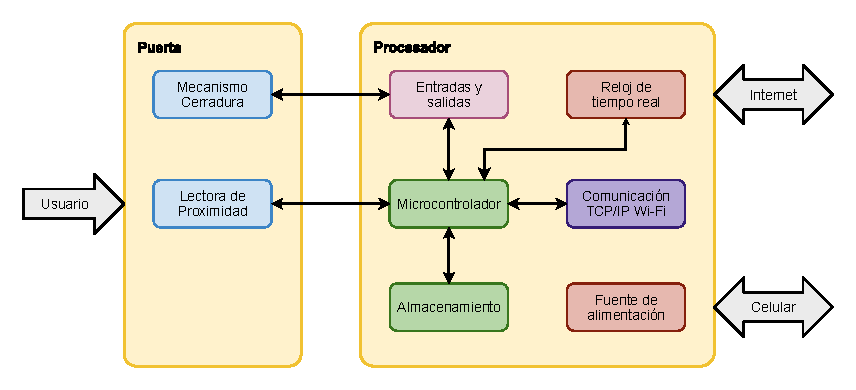
\includegraphics[width=\textwidth]{Figures/BloquesNuevo.pdf}
	\caption{Diagrama de bloques del equipo desarrollado}
	\label{fig:DiagramaBloques}
\end{figure}

\begin{itemize}
	\item Se unificaron las dos unidades funcionales del equipo anterior en el procesador, quedando instalada en la puerta únicamente la placa electrónica que implementa la antena de RFID con el circuito integrado responsable de la generación del campo electromagnético y el procesamiento analógico de la señal recibida. Esto permite además de reducir la cantidad de componentes centralizar en el firmware principal todo el procesamiento de la comunicación con la tarjeta de proximidad.
	\item En el bloque de entradas y salidas se cambió la conexión con el sistema de cerradura para  controlar indistintamente sistemas electromagnéticos o motorizados. Además se agregaron sensores de fin de carrera para el mecanismo de la cerradura, lo que además de aumentar la confiabilidad del sistema permite prolongar la vida útil de los componentes evitando esfuerzos innecesarios.
	\item Se cambió el bloque de comunicaciones Bluetooth por una interfaz WiFi, lo que permitió además adoptar el protocolo TPC/IP para la comunicación con el equipo. Esta interfaz puede operar en modo punto de acceso, lo que permite efectuar una comunicación punto a punto con el celular de la misma forma que se hacía con el Bluetooth. Pero también puede operar en modo estación, de esta forma el equipo puede conectarse una red WiFi existente y permitir la gestión desde cualquier dispositivo autorizado que tenga conexión con esta red.
	\item Se incorpora un reloj de tiempo real independiente del procesador que será el responsable de mantener la fecha y hora del sistema. Este bloque incluye una batería de respaldo que le permite continuar funcionando cuando el equipo no cuenta con alimentación.
\end{itemize}

\section{Prototipo del hardware}
\label{sec:prototipo}

En el diseño de la placa electrónica se siguieron los mismos criterios que ya se mencionaron en la sección \ref{sec:hardware} para la selección de los componentes. Se decidió que mantener el gabinete actual, lo que determinó la geometría de la placa y la posición de la mayoría de los conectores. Se decidió también que la placa se realizaría con las capacidades de fabricación del único fabricante de circuitos impresos de la provincia, a quien se le encomendaría la fabricación del primer prototipo. Con estas restricciones el circuito impreso debía resolverse en dos capas y en un área de 87 x 66 mm. 

El desarrollo de las pistas de cobre no resultó simple, ya que como puede observarse en la figura \ref{fig:BloquesActual} una parte importante del área de la placa se encuentra ocupada por componentes, lo que sumado a la restricción de utilizar pistas de 0,5 mm y vías de 1 mm impuesta por el proceso de fabricación aumentó la dificultad del proceso de diseño. 

\begin{figure}[ht]
	\centering
	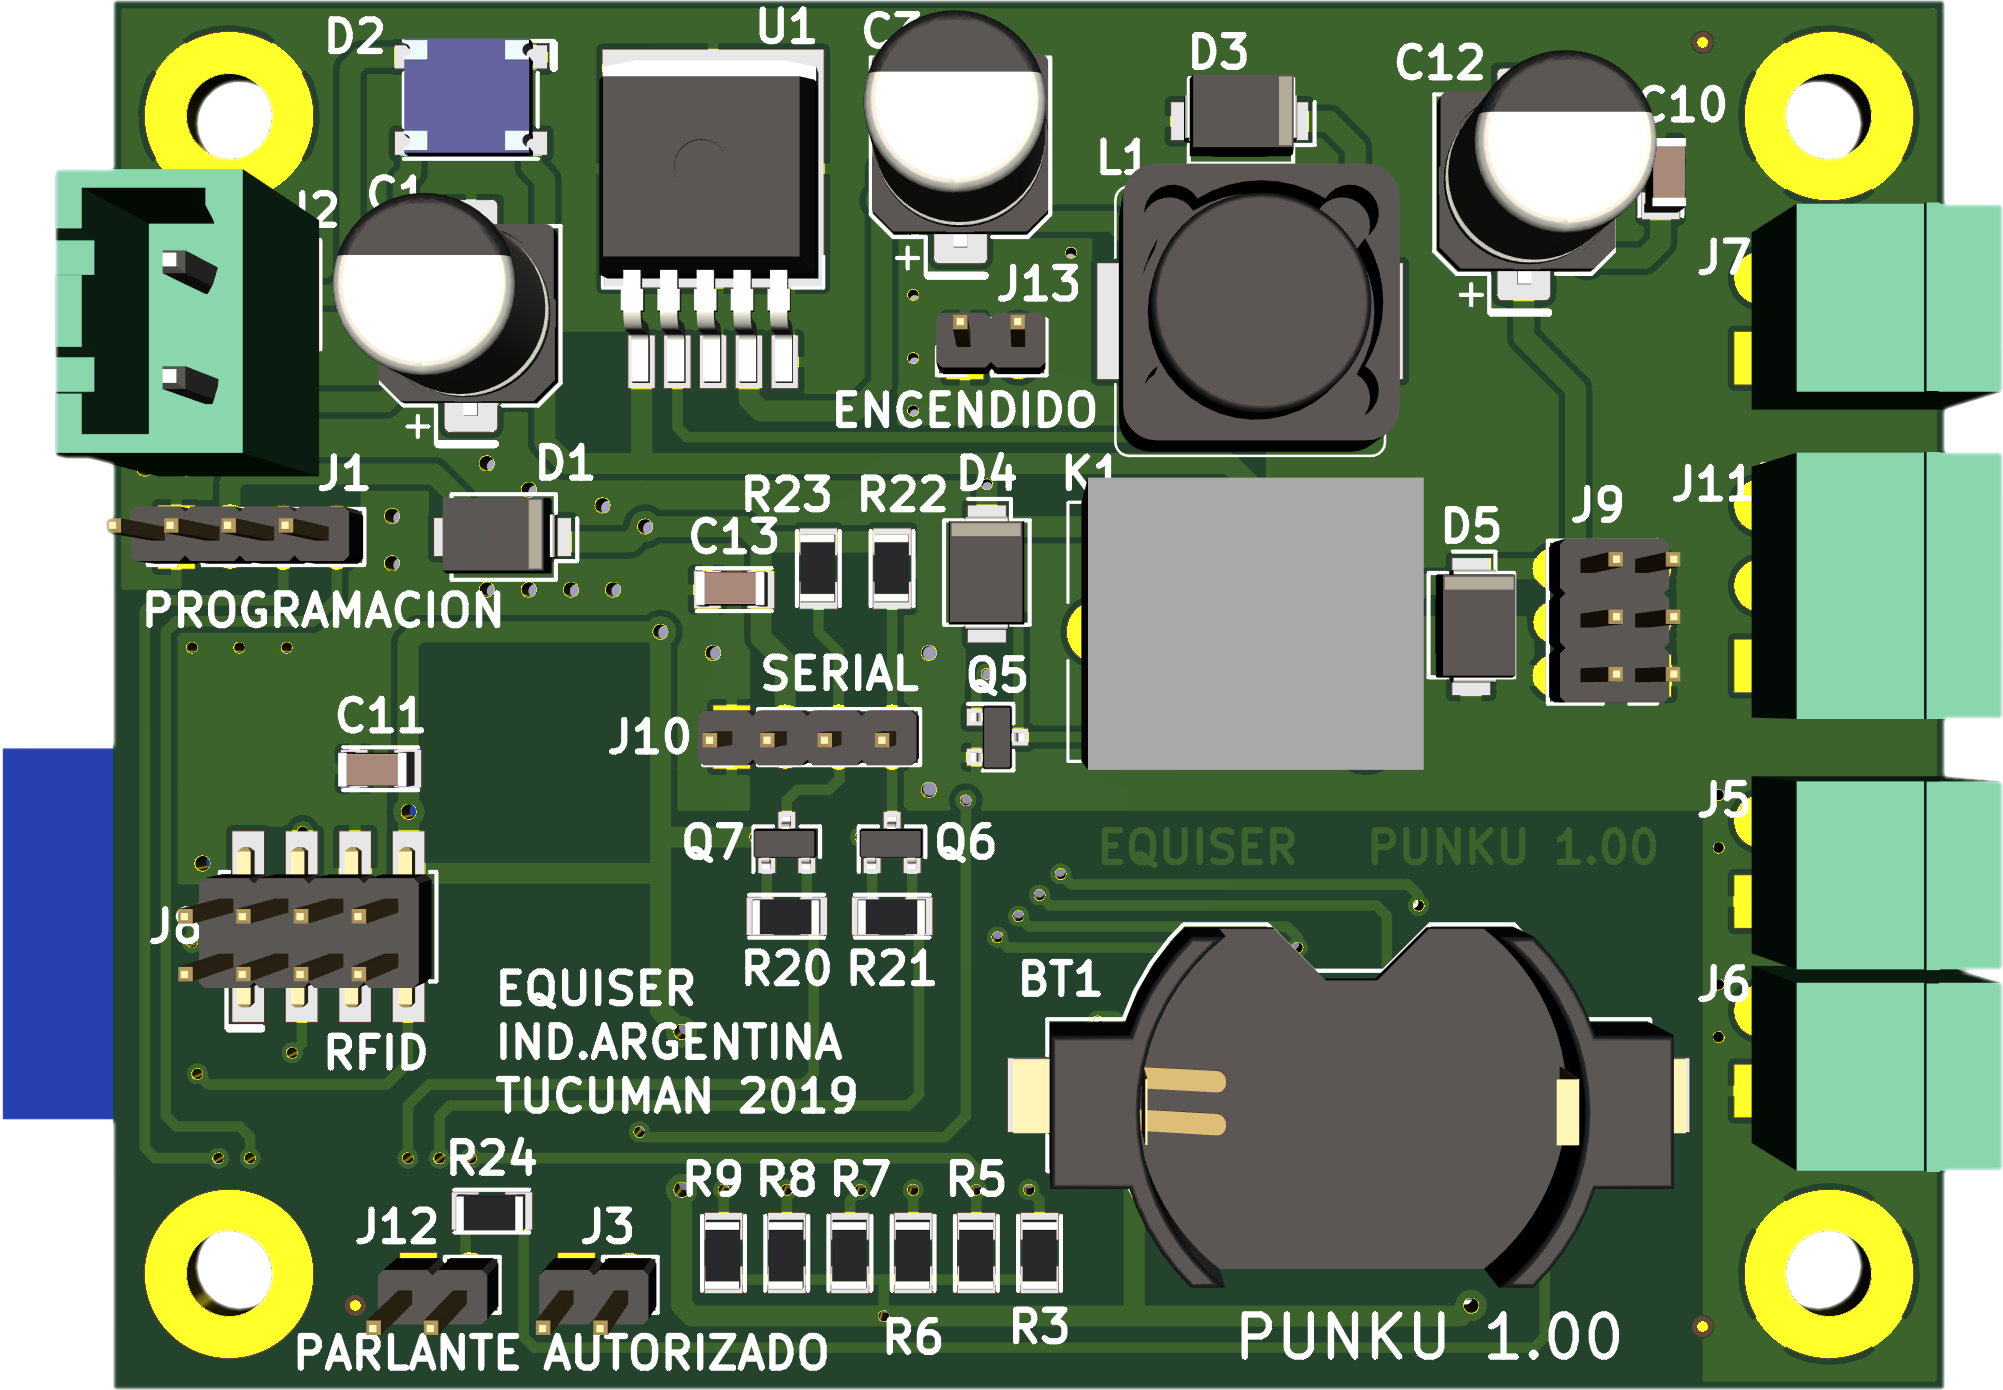
\includegraphics[scale=.15]{Figures/ModeloPlaca.png}
	\caption{Modelo tridimensional de la placa electrónica.}
	\label{fig:Componentes}
\end{figure}

Se efectuó un proceso de doble revisión sobre el diagrama esquemático del circuito y el diseño de la placa, incorporando una serie de recomendaciones efectuadas por los revisores como la utilización de los planos de tierra en las zonas de la placa generadoras de ruido electromagnético. A pesar de las revisiones se encontraron errores en un último control previo al proceso de fabricación de la placa.

El montaje del prototipo se efectuó en forma manual, y durante el mismo se detectaron dificultades para el montaje en algunos componentes. Para resolver estos problemas se efectuaron correcciones en el diseño de la placa, principalmente el aumento de la separación entre los planos de masa y las pistas de señales. En la primera se adoptó un valor similar a la separación entre pistas, pero debido a la falta de precisión en la máscara antisoldante que peude observarse en la imagen \ref{fig:ProblemasMascara}, este valor resultó pequeño y permitió que durante el proceso de soldado se generen puentes de estaño entre los terminales de los componentes y el plano de masa circundante.

\begin{figure}[ht]
	\centering
	\includegraphics[scale=1]{Figures/cuadradoAzul.png}
	\caption[Problemas con la  máscara antisoldante del prototipo]{Imagen que muestra la falta de precisión en la aplicación de la máscara antisoldante del prototipo.}
	\label{fig:ProblemasMascara}
\end{figure}

\section{Diseño del firmware}
\label{sec:firmware}

\subsection{Arquitectura del firmware}

Uno de los objetivos planteados para el trabajo en la sección \ref{sec:objetivos} fue la reingeniería completa del firmware del equipo, que permita incorporar el uso de un sistema operativo de tiempo real y el reuso de los componentes comunes en otros proyectos similares. Para esto se decidió utilizar una arquitectura de capas, la cual se puede observar en el diagrama de componentes de la figura \ref{fig:DiagramaComponentes}. En la misma se pueden identificar claramente cuatro capas:

\begin{figure}[ht]
	\centering
	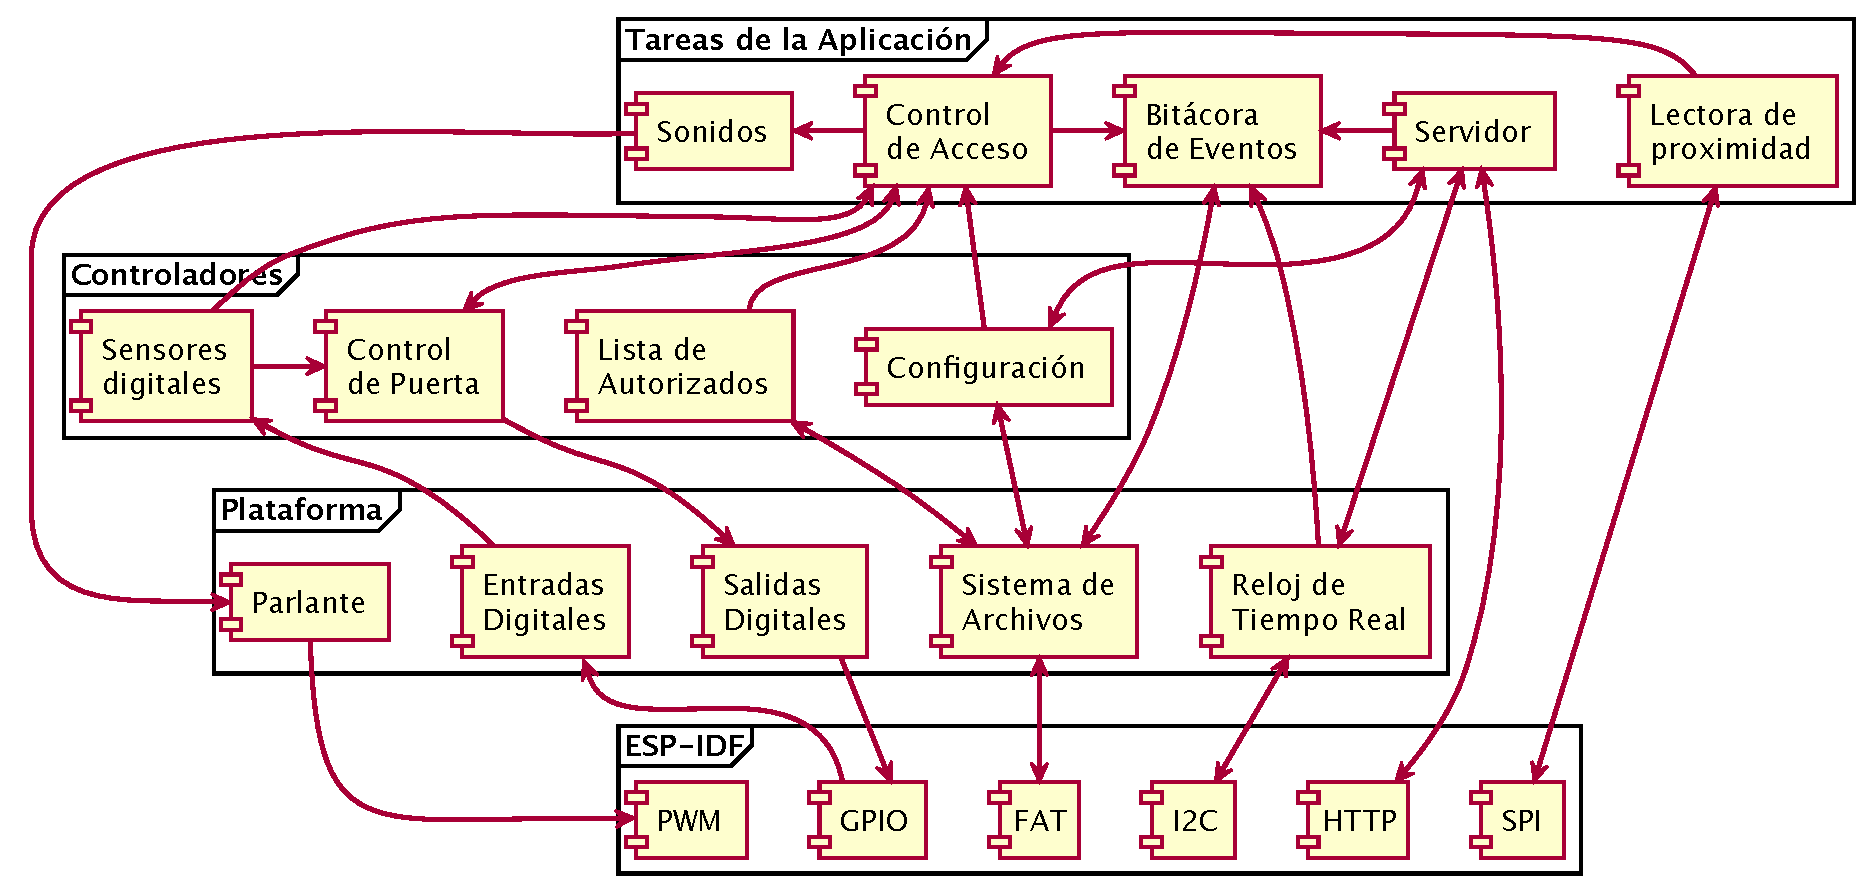
\includegraphics[width=\textwidth]{./Figures/PNK-DC001.pdf}
	\caption{Diagrama de componentes del firmware del equipo}
	\label{fig:DiagramaComponentes}
\end{figure}

\begin{itemize}
	\item ESP-IDF: corresponde al conjunto de funciones provistas por el fabricante para facilitar el desarrollo en la plataforma. En la misma se incluyen los controladores para los puertos GPIO, SPI, I2C y PWM. También se incluye la implementación del sistema de archivos FAT para tarjetas SD y de un servidor HTTP completo.

	\item Plataforma: implementa una capa de abstracción del hardware, también conocida como \emph{Hardware Abstraction Layer} (HAL), que permite independizar el resto del código desarrollado de la plataforma provista por el fabricante. Esta capa facilita la reutilización del resto de los componentes en proyectos similares y la eventual migración del firmware a otra plataforma.

	\item Controladores: implementa una serie de clases que se pueden reutilizar en otros proyectos fácilmente ya que no dependen del hardware ni de la aplicación.

	\item Aplicación: implementa la lógica propia del equipo mediante un conjunto de tareas que ejecutan concurrentemente en un sistema operativo de tiempo real.
\end{itemize}

Para el modelado de los componentes se utilizó el análisis orientado a objetos, lo que arrojo como resultado una colección de clases con sus respectivos métodos y atributos. Una imagen completa de este diseño se puede observar en el diagrama de clases que se muestra en la figura \ref{fig:DiagramaClases}. En el mismo solo están incluidos los componentes de las tres clases superiores desarrolladas en el marco del trabajo. En las siguientes subsecciones se explican brevemente las responsabilidades asignadas a cada una de estas clases.

\begin{figure}[ht]
	\centering
	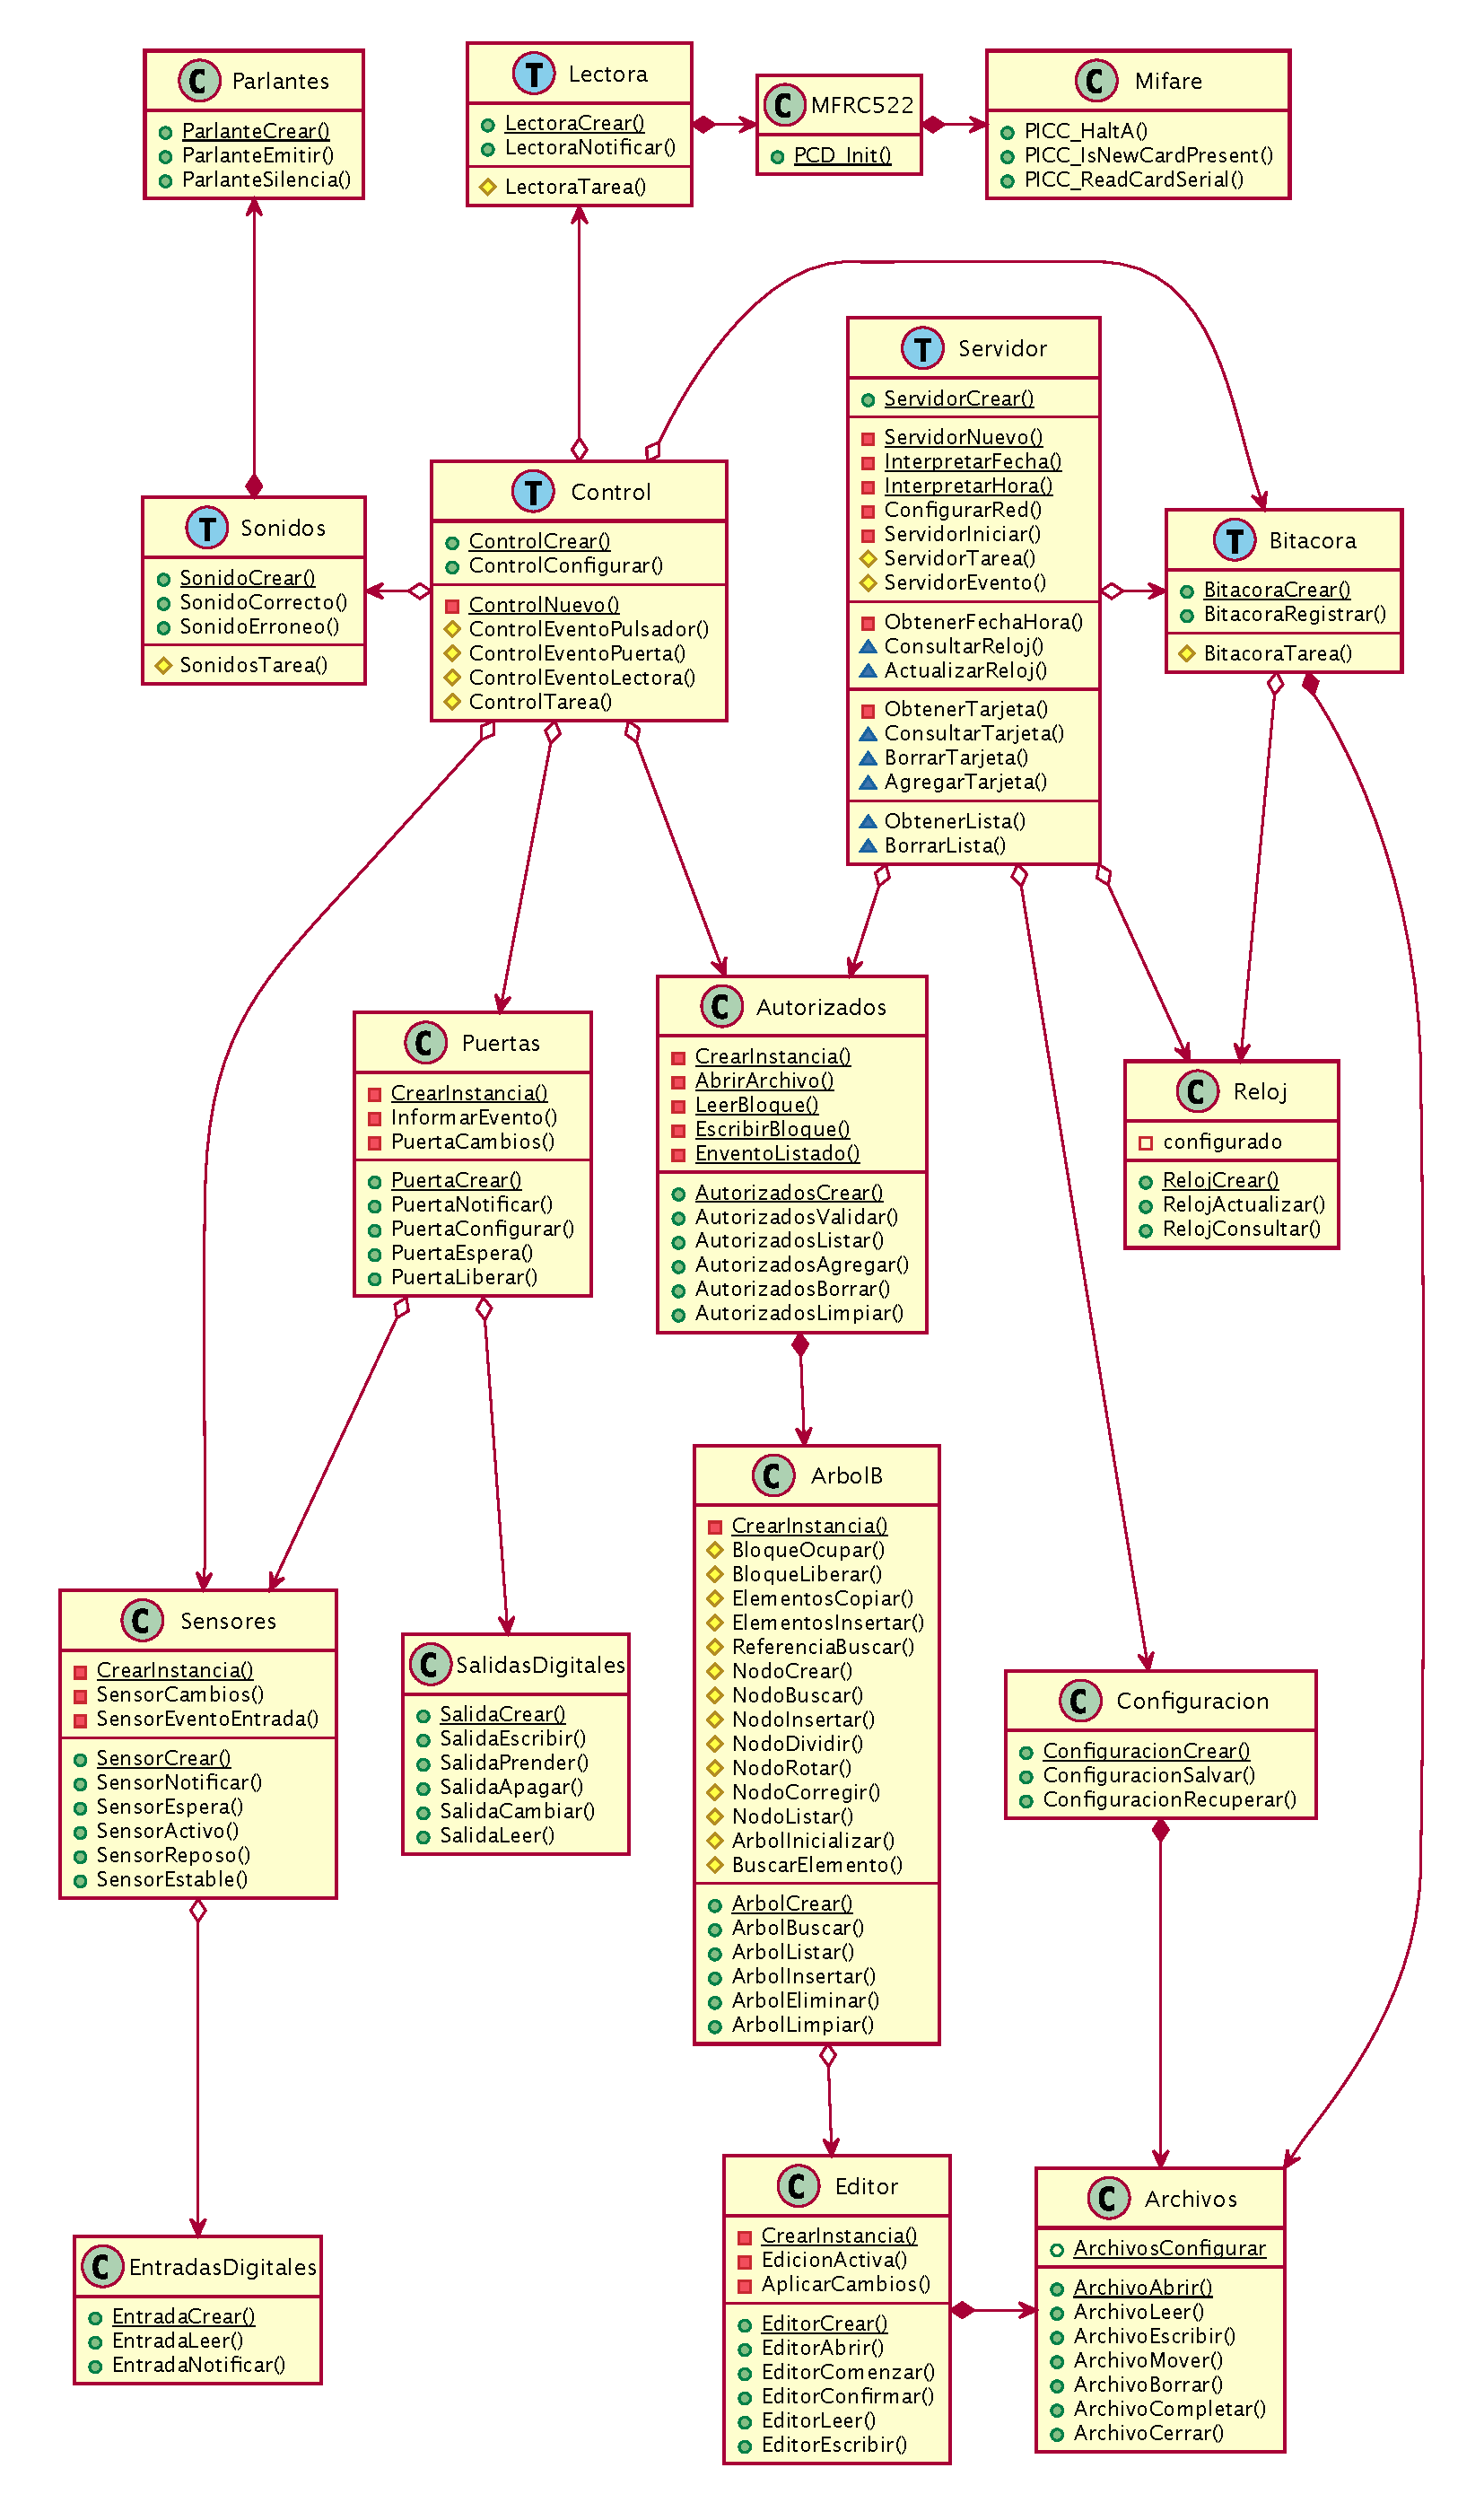
\includegraphics[width=\textwidth]{./Figures/PNK-DC002.pdf}
	\caption{Diagrama de clases del firmware del equipo}
	\label{fig:DiagramaClases}
\end{figure}

\subsection{Capa de abstracción del hardware}

Esta capa contiene una colección de clases que encapsulan las funcionalidades del entorno de desarrollo provisto por el fabricante. El principal objetivo de las mismas es brindar una plataforma uniforme en comportamiento y documentación para el resto del firmware. Las clases que pertenecen a esta capa son:

\begin{itemize}
	\item EntradasDigitales: encapsula toda la gestión de un terminal digital utilizado como entrada. Permite configurarlo durante la creación del objeto, recuperar el estado actual y solicitar el envío de eventos generados por interrupciones disparadas por cambios en el estado del mismo.
	
	\item SalidasDigitales: encapsula toda la gestión de un terminal digital utilizado como salida. Permite configurarlo durante la creación del objeto, recuperar el estado actual y cambiarle el estado.
	
	\item Archivos: encapsula toda la gestión de un archivo almacenado en la tarjeta microSD del equipo. Después de la configuración de la propia clases permite la creación y el borrado de archivos, como así también la escritura y lectura de datos en los mismos.
	
	\item Reloj: encapsula toda la gestión del reloj de tiempo real. Permite ajustar y recuperar la fecha y hora actuales.
	
	\item Parlantes: encapsula la gestión de un parlante conectado a un terminal digital que opera con modulación de ancho de pulso, o \emph{Pulse Width Modulation} (PWM). Permite emitir un tono  generando una señal cuadrada de frecuencia arbitraria o silenciarlo.
\end{itemize}

\FloatBarrier

\subsection{Capa de controladores}

Las clases que componen esta capa son independientes de la plataforma y de la aplicación, y por lo tanto son fácilmente reutilizables en otros proyectos. Para lograr este objetivo, la mayoría de ellas no utilizan  los servicios del sistema operativo, e implementan mecanismos de eventos para  extraer el código dependiente de la aplicación en otro componente. Las clases que pertenecen a esta capa son:

\begin{itemize}
	\item Puertas: encapsula toda la gestión de la puerta. Permite configurar el tipo de cerradura, habilitar o ignorar el sensor de puerta abierta y definir los tiempos correspondientes de liberación, apertura y cierre. Puede generar eventos cuando se completa un ciclo de apertura. Esta clase tiene una especial importancia en el sistema, ya que la misma implementa aproximadamente el 30\% de los requisitos funcionales definidos en la sección \ref{sec:Requisitos}. Para la implementación se optó por utilizar cuatro maquinas de estado finitos independientes, una para cada modo de funcionamiento descrito en la tabla \ref{tab:ModosOperacion}. Para modelar las mismas se utilizaron diagramas de estado UML, los cuales se pueden ver en las figuras \ref{fig:ControlSinSin}, \ref{fig:ControlSinCon}, \ref{fig:ControlConSin} y \ref{fig:ControlConCon}

\begin{figure}[ht]
	\centering
	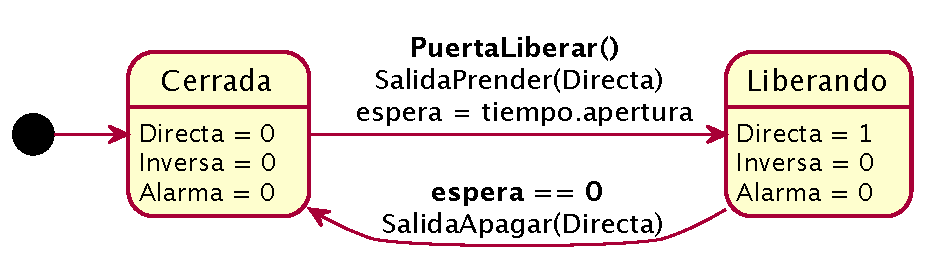
\includegraphics[scale=.5]{Figures/PNK-DE001.pdf}
	\caption{Diagrama de estado para el control de una puerta, sin sensor de apertura y con liberación electromagnética}
	\label{fig:ControlSinSin}
\end{figure}

\begin{figure}[ht]
	\centering
	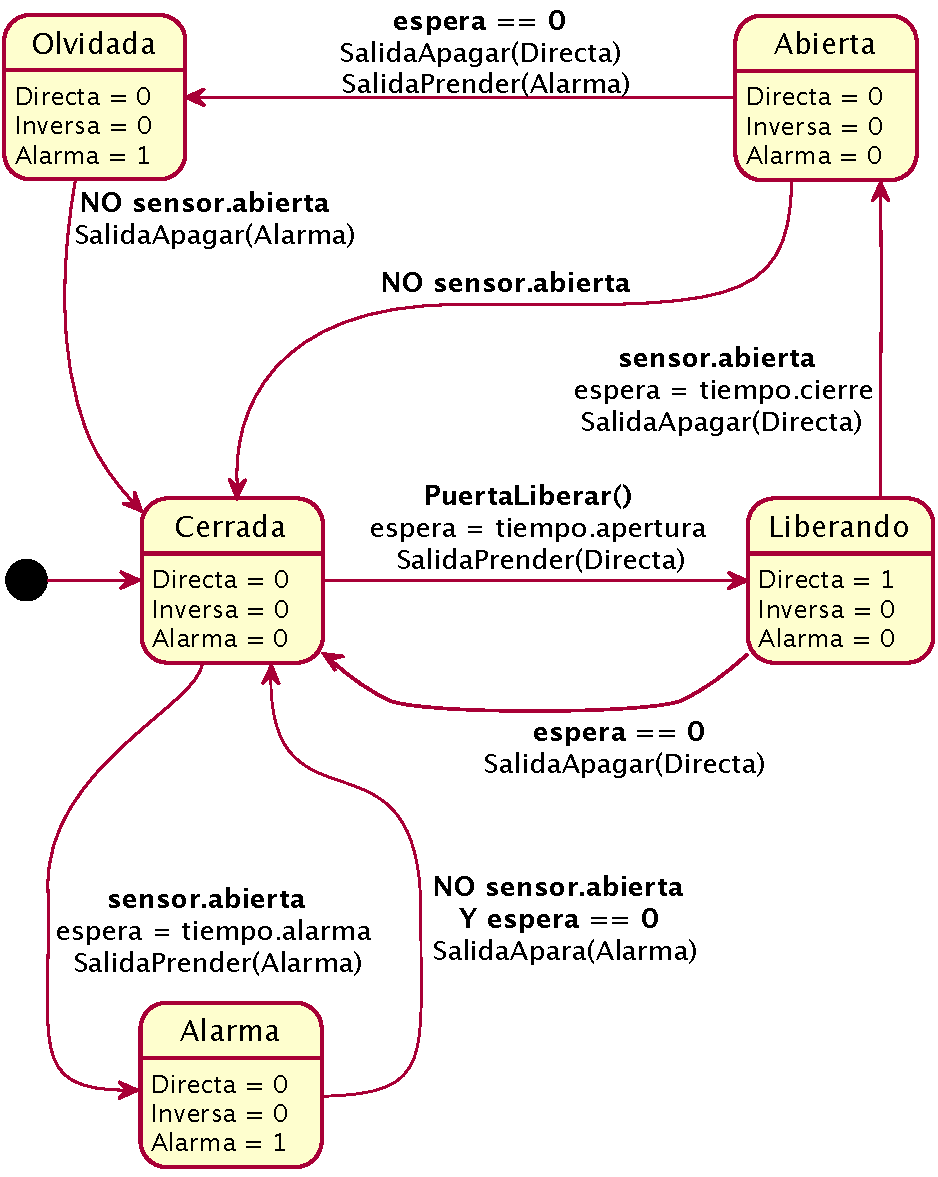
\includegraphics[scale=.5]{Figures/PNK-DE002.pdf}
	\caption{Diagrama de estado para el control de una puerta, con sensor de apertura y con liberación electromagnética}
	\label{fig:ControlSinCon}
\end{figure}

\begin{figure}[ht]
	\centering
	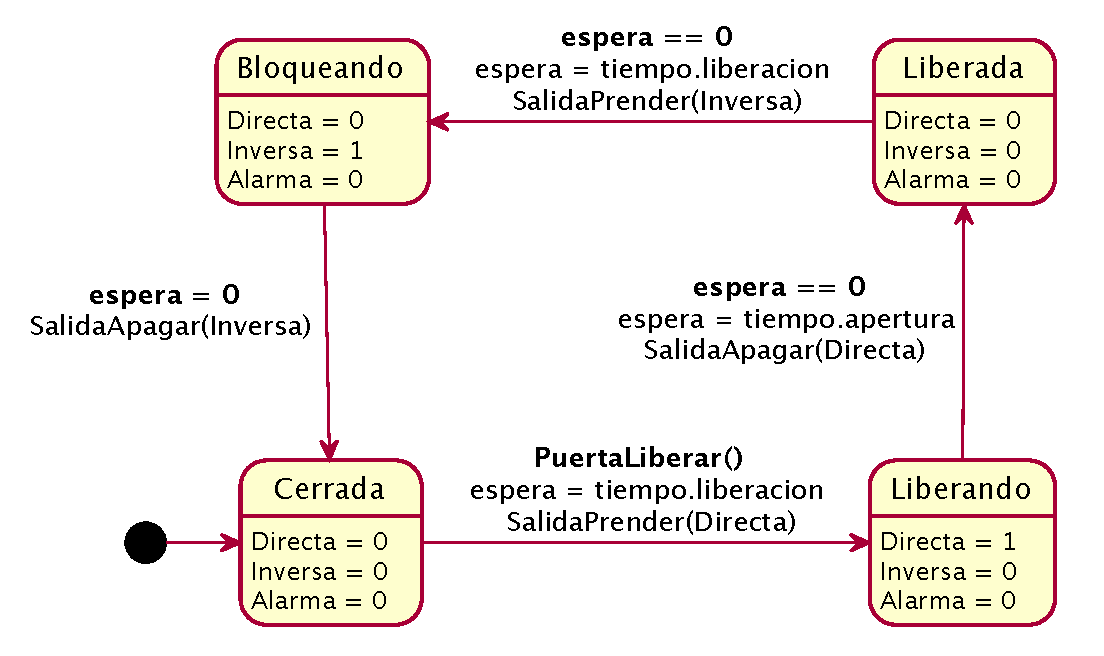
\includegraphics[scale=.5]{Figures/PNK-DE003.pdf}
	
	\caption{Diagrama de estado para el control de una puerta, sin sensor de apertura y con liberación motorizada}
	\label{fig:ControlConSin}
\end{figure}

\begin{figure}[ht]
	\centering
	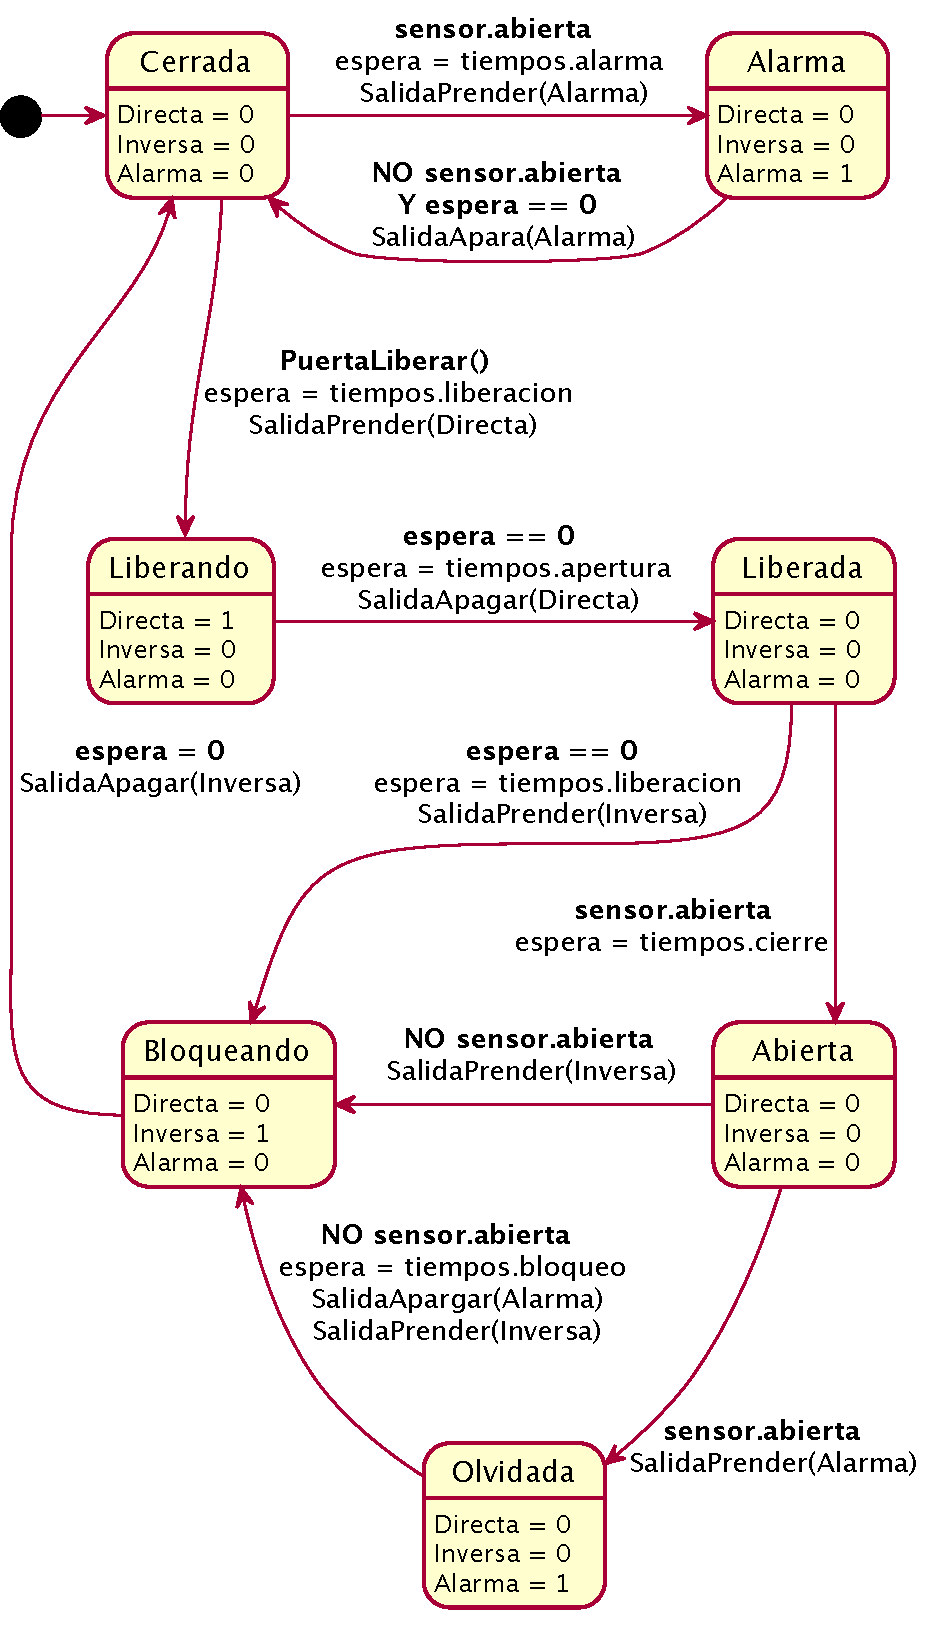
\includegraphics[scale=.5]{Figures/PNK-DE004.pdf}
	\caption{Diagrama de estado para el control de una puerta, con sensor de apertura y con liberación motorizada}
	\label{fig:ControlConCon}
\end{figure}

\FloatBarrier
	
	\item ArbolB: encapsula toda la gestión de un índice utilizando la estructura de datos denominada ArbolB  o \emph{BTree}. Permite aprovechar las transferencias de bloques en los almacenamientos secundarios, como la tarjeta microSD, para disminuir el tiempo de búsqueda y actualización de una lista ordenada. Esta clase junto con la clase junto con la clase Editor que se explica a continuación son también componentes críticos del sistema, ya que cualquier error en ellas se traduce en personas autorizadas que no pueden ingresar, o peor aún, en accesos de personas no autorizadas. Pero a diferencia de la clase Puertas, en estas clases el aspecto crítico está en la implementación y no en el diseño, ya que los algoritmos que utilizan las dos clases son ampliamente conocidos.
		
	\item Editor: encapsula toda la gestión de una actualización que involucra múltiples escrituras en un archivo. Permite asegurar que el contenido del índice de tarjetas autorizadas no resultará corrupto por una modificación incompleta. Esta clase utiliza el concepto de transacción \emph{ACID (Atomicity, Consistency, Isolation and Durability)} muy común en las bases de datos relacionales, que en nuestro caso se puede resumir en que cualquier cambio al índice se realiza siempre de manera completa, o de lo contrario, no efectúa absolutamente ningún cambio. Para la implementación se utilizó un archivo de transacciones donde se registran las escrituras de los sectores que se van actualizando en el índice. Al completar la modificación esta se confirma en el mismo archivo de transacciones, y a partir de este punto se comienzan a aplicar los cambios en el archivo de datos. Si ocurre una interrupción del proceso, por ejemplo por un reinicio del sistema, primer se buscan transacciones confirmadas para aplicar los cambios nuevamente y recién se comienza la operación del sistema.

	\item Autorizados: encapsula toda la gestión de una lista con las tarjetas autorizadas a ingresar. Permite consultar si una tarjeta esta autorizada, recuperar toda la lista de tarjetas autorizadas y agregar o eliminar una tarjeta en ella. Esta clase agrega muy poca lógica y es prácticamente un adaptador de la clase ArbolB para convertir la funcionalidad de un índice en una lista presente/ausente. Esta clase agrega además el control de sección crítica necesario para que el indice pueda ser consultado y actualizado por dos tareas diferentes que ejecutan en forma concurrente.

	\item Sensores: encapsula toda la gestión de filtro digital asociado a terminales digitales de entrada. Permite definir un valor de histéresis para eliminar los eventos generados por ruido electromagnético. También permite generar eventos por cambios en el estado del mismo y determinar si la entrada digital presenta un estado estable o se encuentra en transición.

	\item Configuración: encapsula toda la gestión de las opciones de configuración del equipo. Permite consolidar las opciones que pueden cambiar en cada uno de los componentes en una estructura binaria, la cual puede ser convertida desde y hacia una cadena de caracteres utilizando la codificación JSON.
\end{itemize}


\subsection{Tareas del sistema}

En esta capa se encuentran las clases que implementan directamente la lógica de funcionamiento del equipo con el  mayor nivel de abstracción. Esto permite extender la funcionalidad en forma simple, dado que el código de las mismas aplica casi directamente las reglas de negocio del equipo. Todas las clases de esta capa encapsulas tareas del sistema operativo de tiempo real que se ejecutan en forma concurrente. Las clases que componen esta capa son:

\begin{itemize}
	\item Sonidos: encapsula toda la reproducción de una melodía monofónica en un parlante. Define una secuencia de notas especificando la frecuencia y duración de las mismas, y de esta manera permite generar dos sonidos distintivos para diferencias los accesos autorizados de los rechazados.
	
	\item Lectora: encapsula toda la comunicación con la lectora y, por medio de esta, con la tarjeta de proximidad. Permite recuperar el número de serie único asignado a la tarjeta y genera un evento al control para informar de una nueva lectura.

	\item Control: encapsula toda la gestión de las reglas para la apertura y supervisión de la puerta. Esta clase implementa un patrón de diseño de software denominado control ambiental, de esta forma convergen en un solo punto los eventos de la clase Puerta, de la clase Sensor, de la clase Lectora y de la clase Autorizados para centralizar la respuesta y el registro a estos eventos. 
	
	\item Bitacora: encapsula el proceso de registro en un archivo de los eventos generados por el control. Permite efectuar la escritura en el archivo, una operación lenta, en forma diferida para minimizar la interferencia en los tiempos de operación del control de la puerta.
	
	\item Servidor: encapsula todo el servicio de comunicación para la gestión del equipo. Permite configurar la interfaz WiFi, iniciar un servidor HTTP y atender los pedidos recibidos interactuando con las clases Reloj, Bitacora, Configuracion y Autorizados para completar las operaciones solicitadas.
	
\end{itemize}

De la descripción anterior se desprende que la correcta interacción entre las clases de esta capa resulta clave para que lograr el correcto funcionamiento del equipo. La ingeniería de software nos brinda una herramienta para poder representar estas interacciones entre los componentes de un programa: los diagramas de secuencia UML. En los mismos se representan las llamadas a métodos de las diferentes clases siguiente los casos de uso analizados en la subsección \ref{sub:CasosDeUso} .Los diagramas más importantes pueden verse en las figuras \ref{fig:SecuanciaPulsador}, \ref{fig:SecuenciaTarjeta}, \ref{fig:SecuenciaForzada} y \ref{fig:SecuenciaConfiguracion}

\begin{figure}[ht]
	\centering
	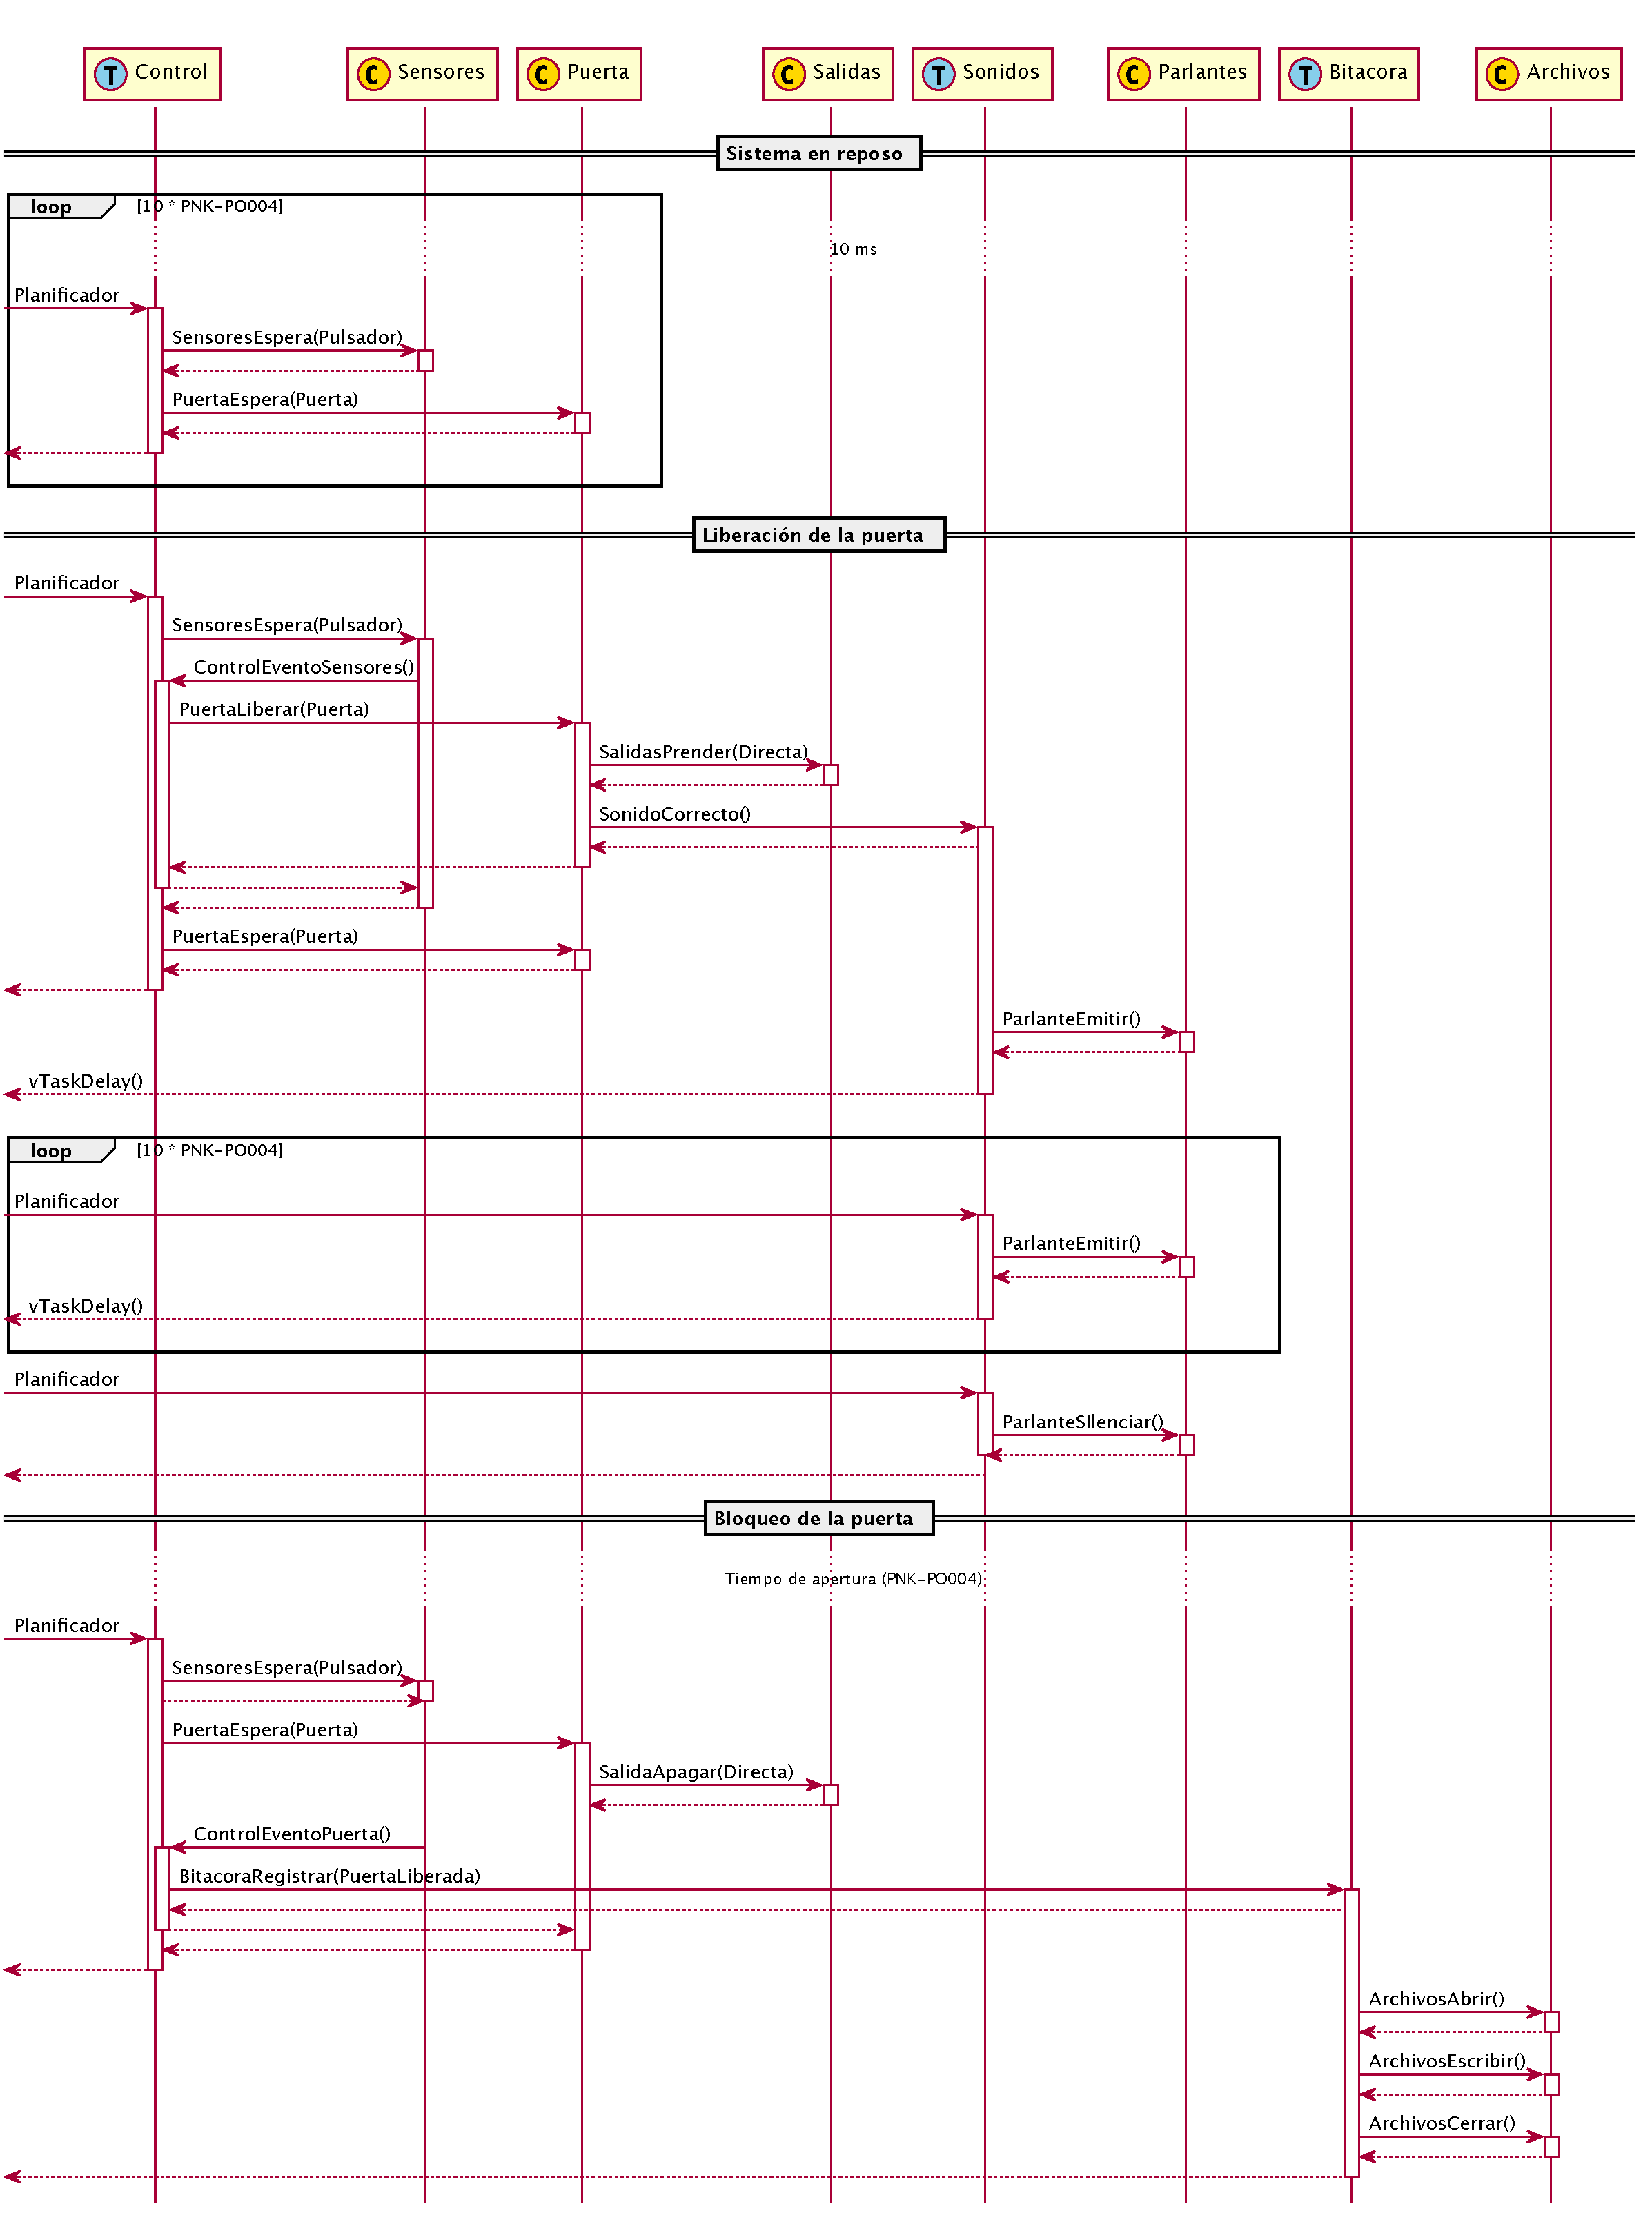
\includegraphics[width=\textwidth]{Figures/PNK-DS001.pdf}
	\caption{Diagrama de secuencia para la liberación por pulsador de una puerta, sin sensor de apertura y con liberación electromagnética}
	\label{fig:SecuanciaPulsador}
\end{figure}

\begin{figure}[ht]
	\centering
	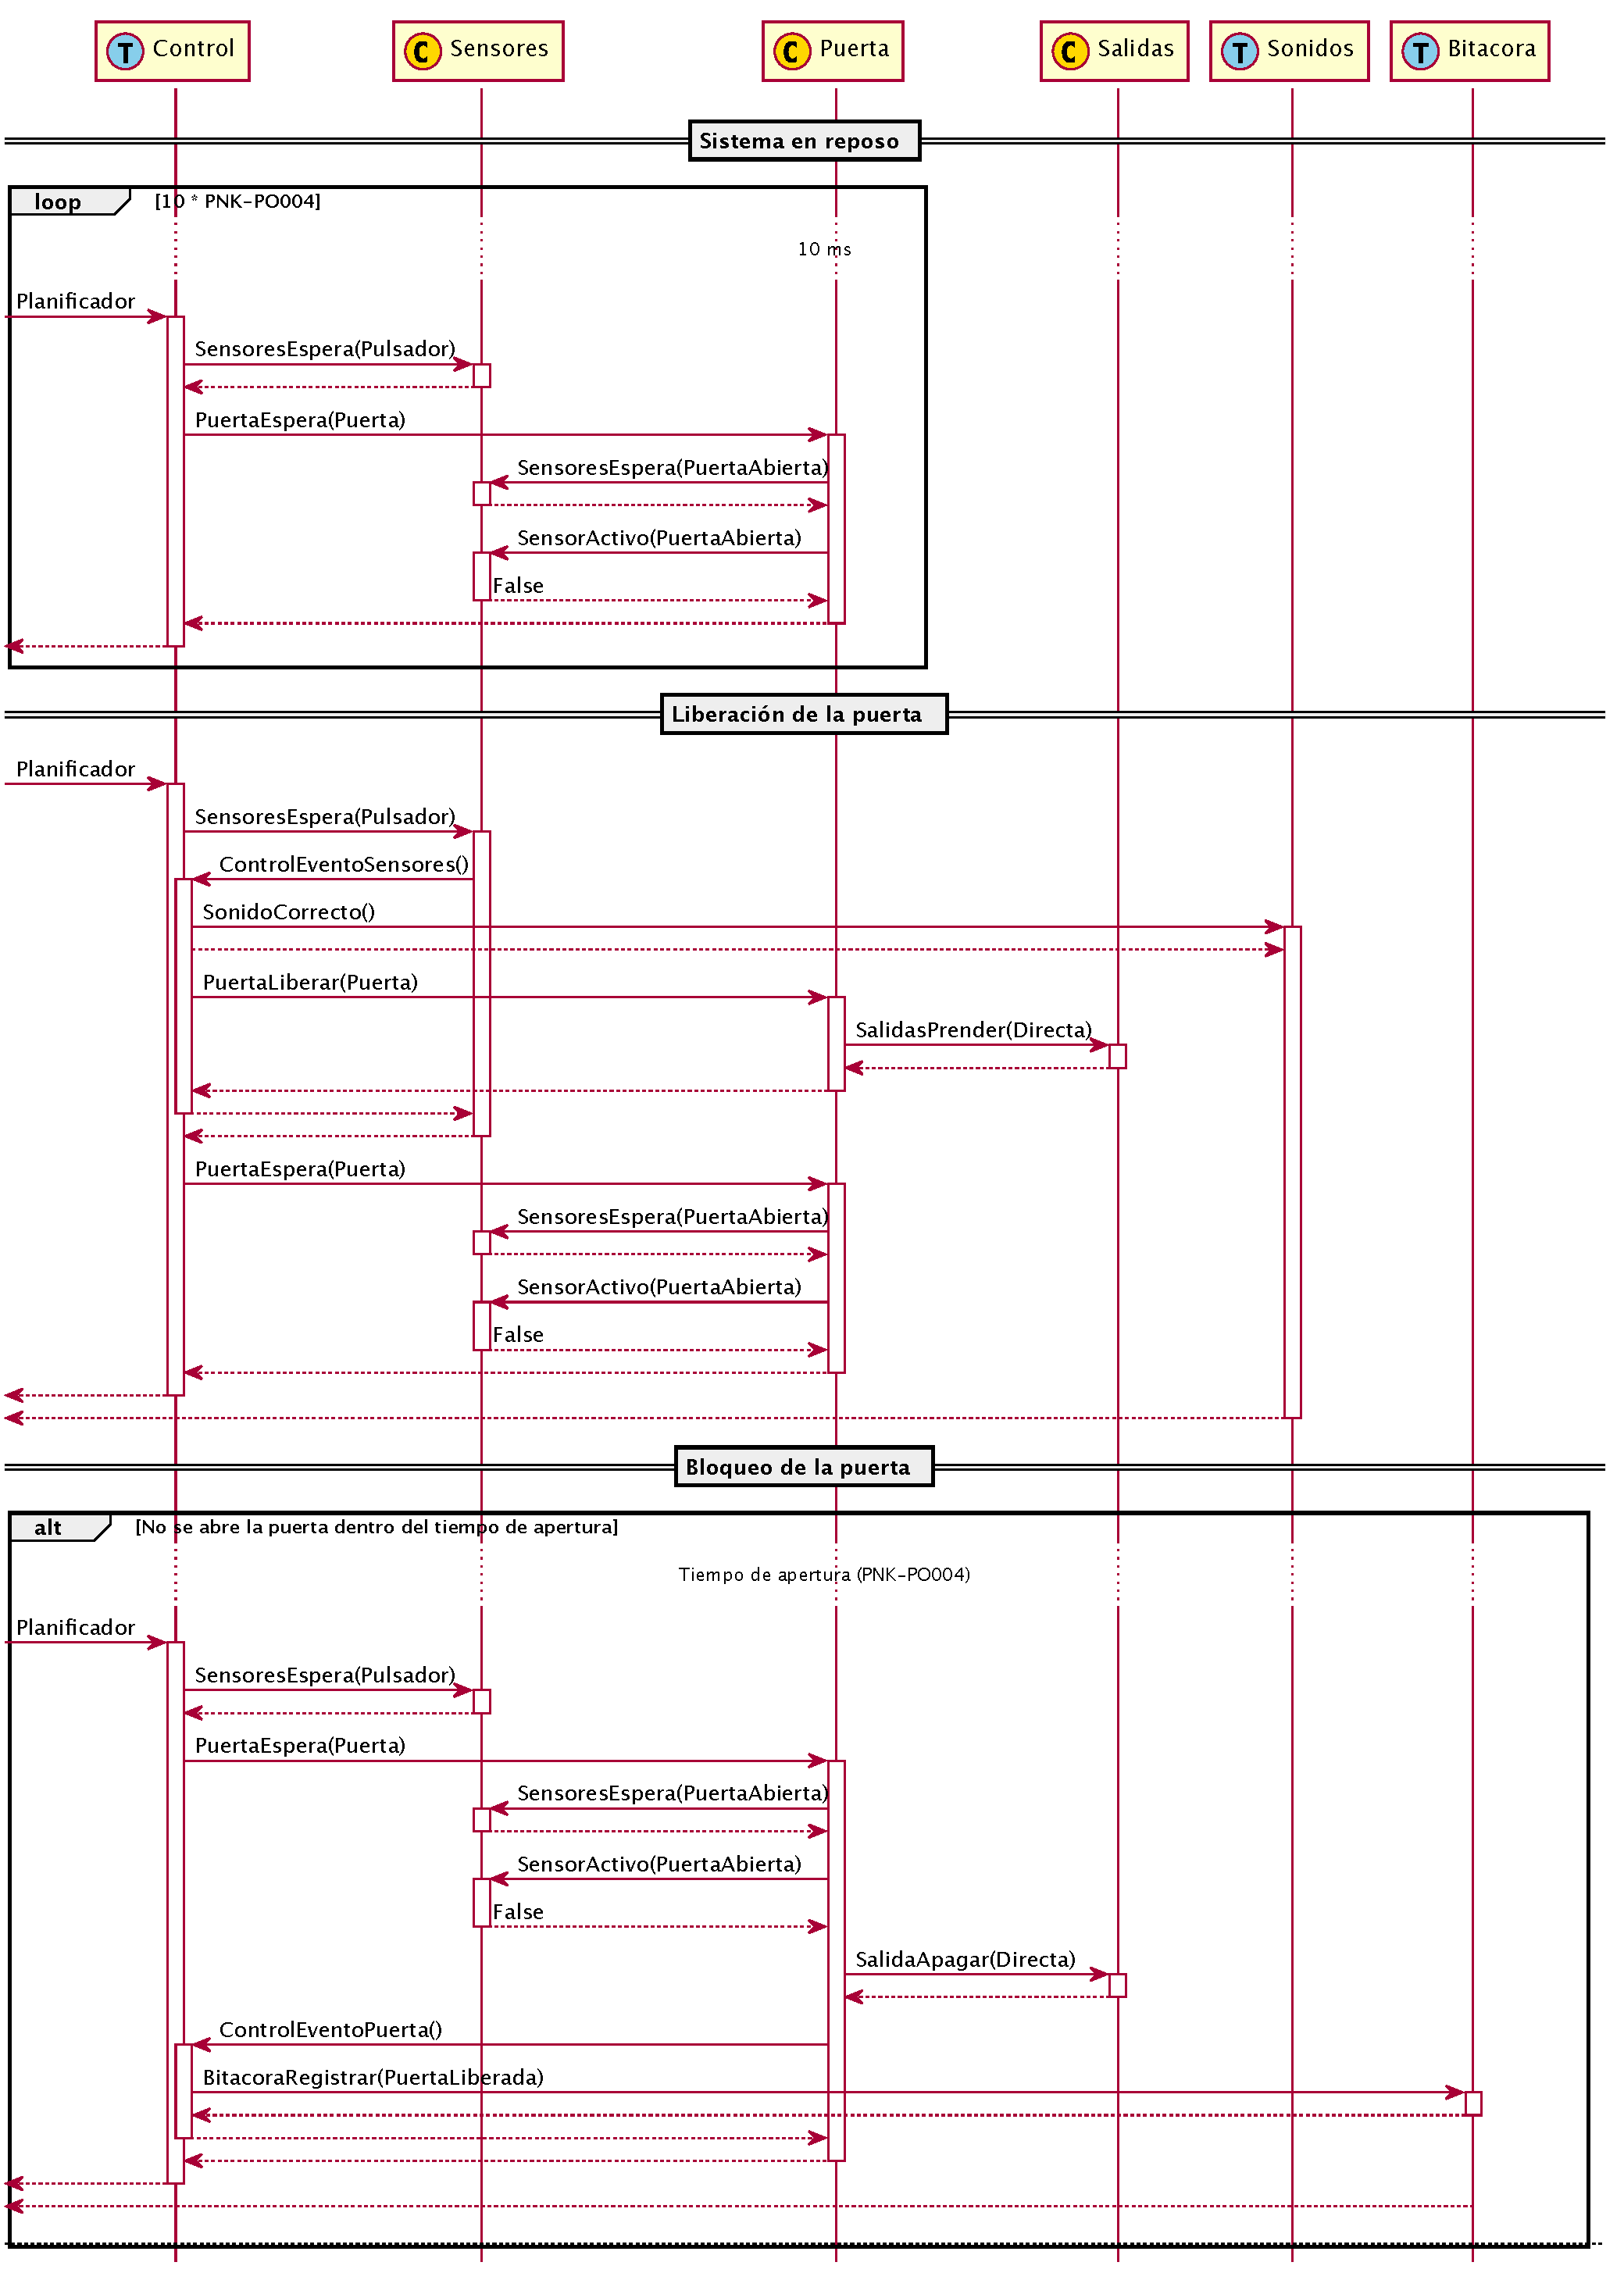
\includegraphics[width=\textwidth]{Figures/PNK-DS002-A.pdf}
	{\color{red} No es el diagrama correcto pero tiene la misma forma y extensión}
	\caption{Diagrama de secuencia para la apertura y cierre por tarjeta de proximidad, con sensor de apertura y con liberación electromagnética}
	\label{fig:SecuenciaTarjeta}
\end{figure}

\begin{figure}[ht]
	\centering
	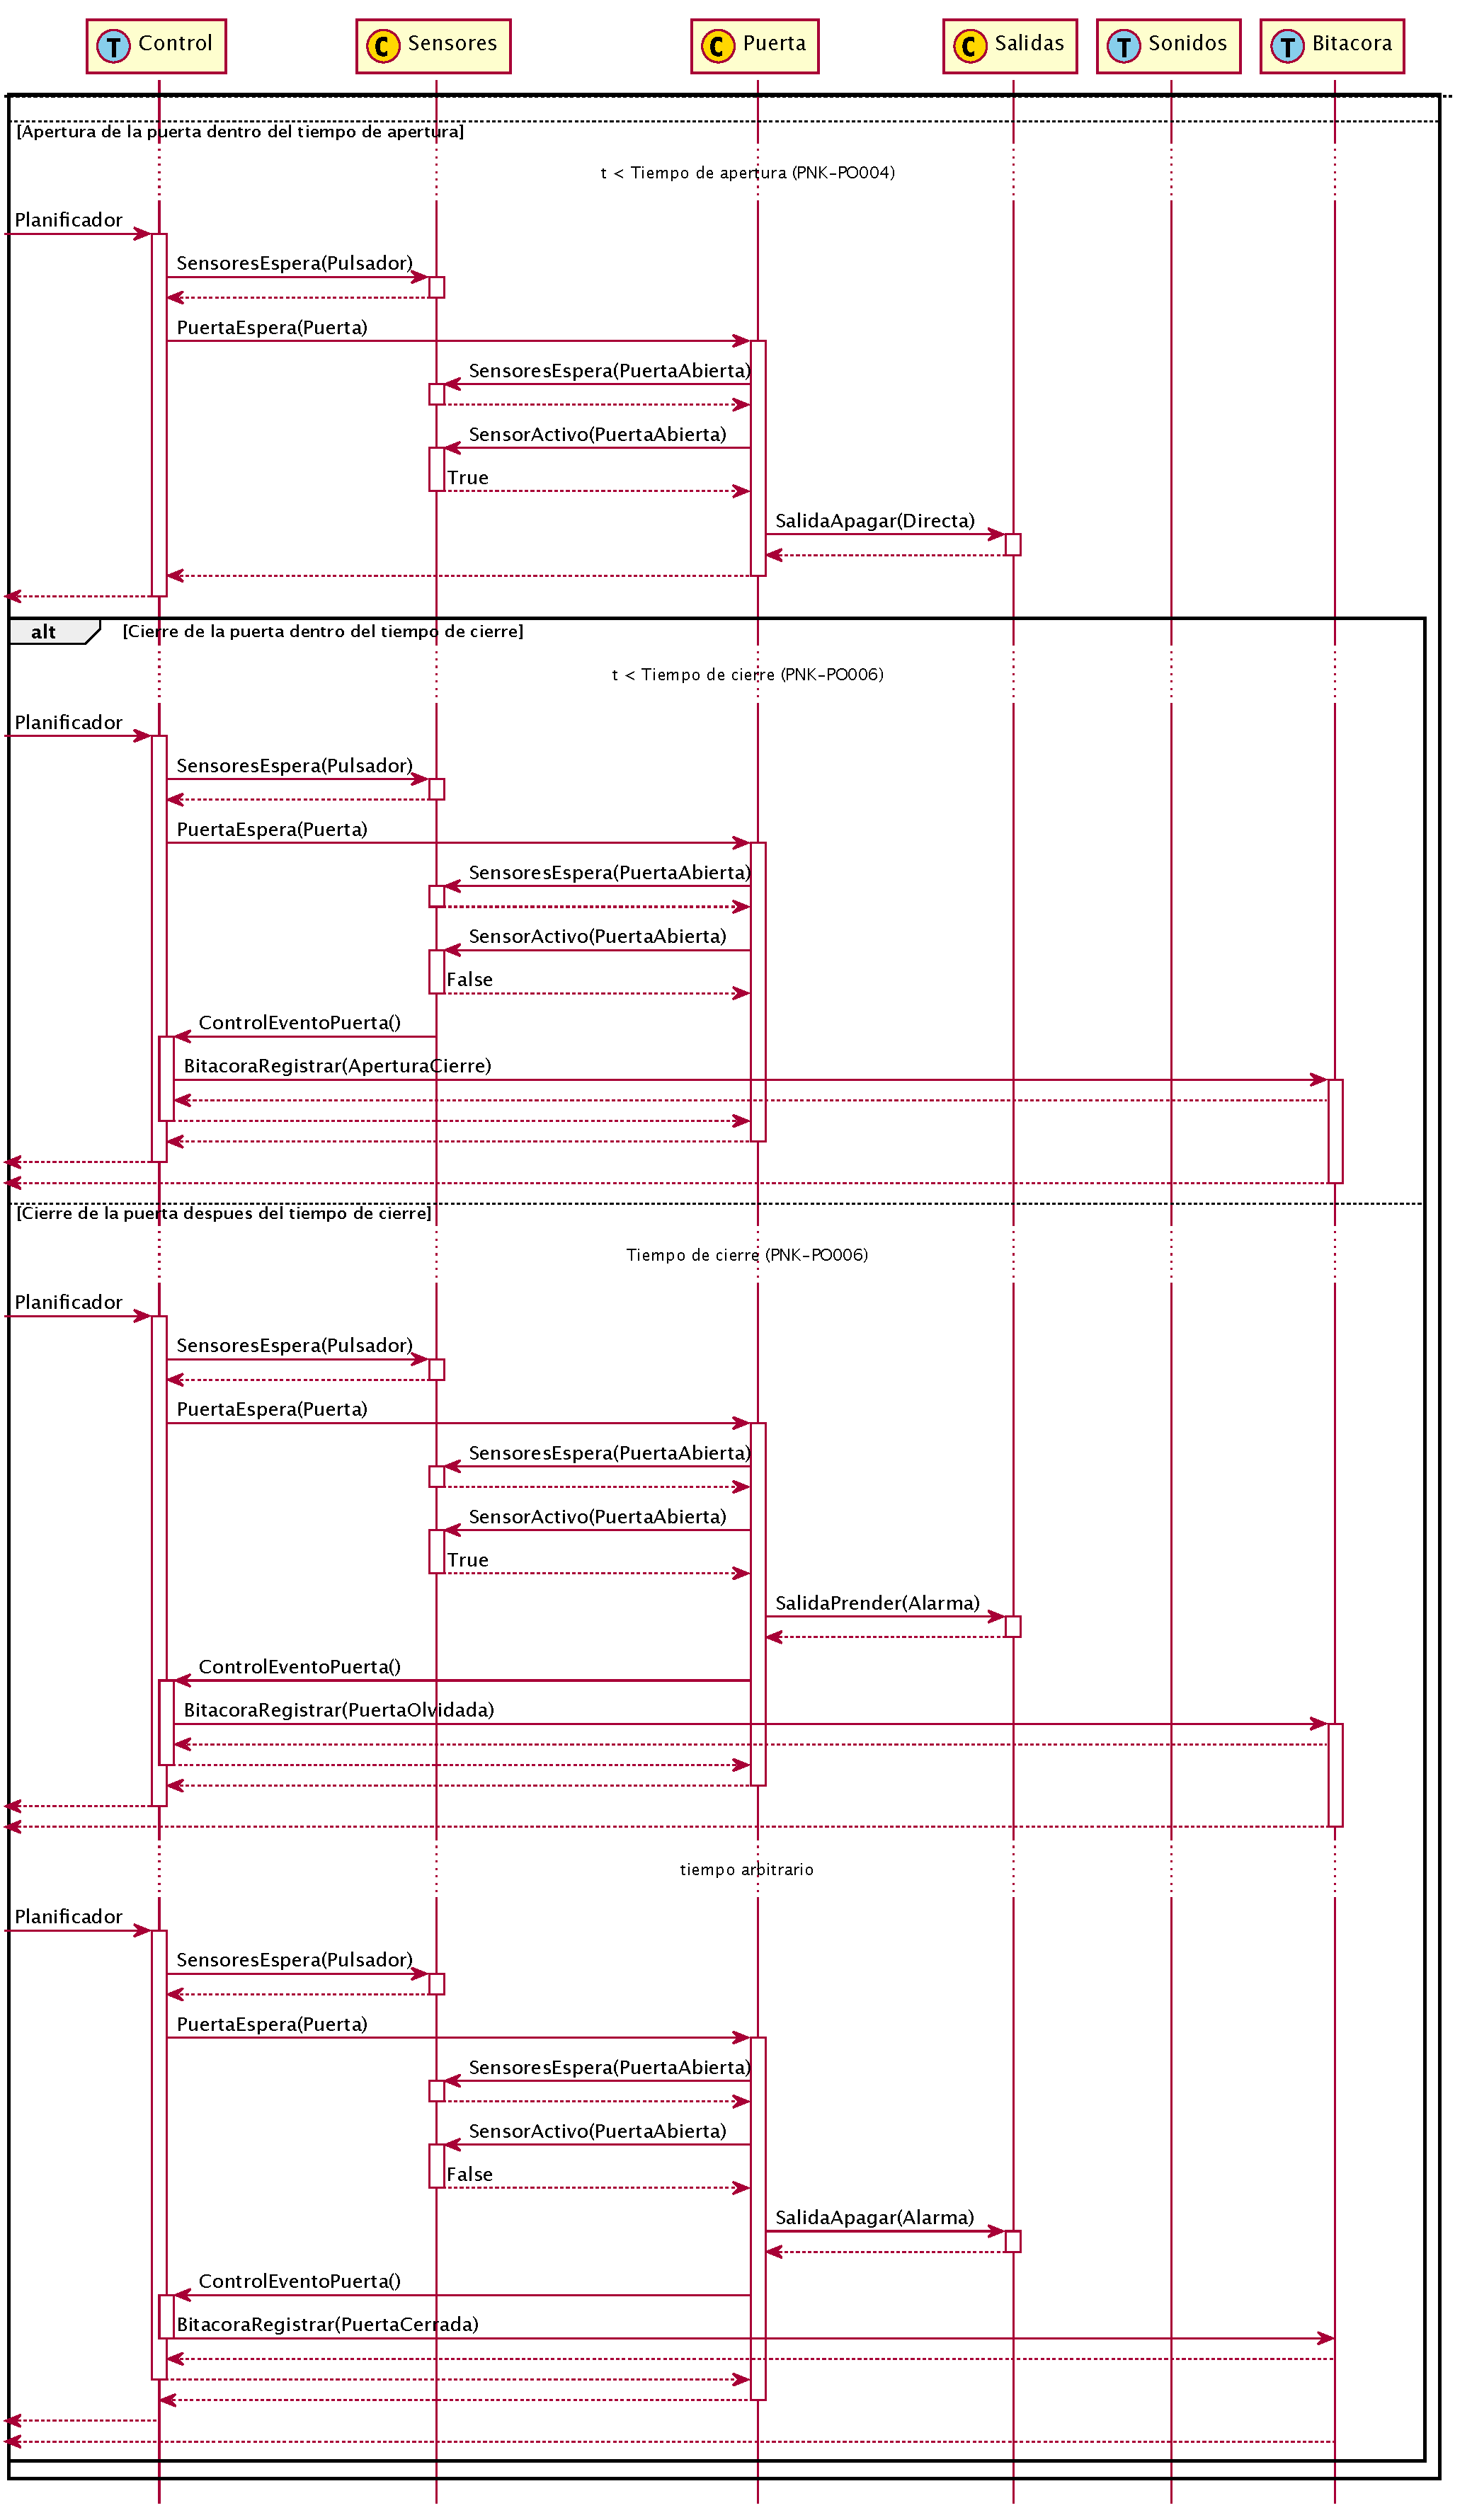
\includegraphics[width=\textwidth]{Figures/PNK-DS002-B.pdf}
	{\color{red} No es el diagrama correcto pero tiene la misma forma y extensión}
	\caption{Diagrama de secuencia para la activación de alarma por apertura forzada de la puerta}
	\label{fig:SecuenciaForzada}
\end{figure}

\begin{figure}[ht]
	\centering
	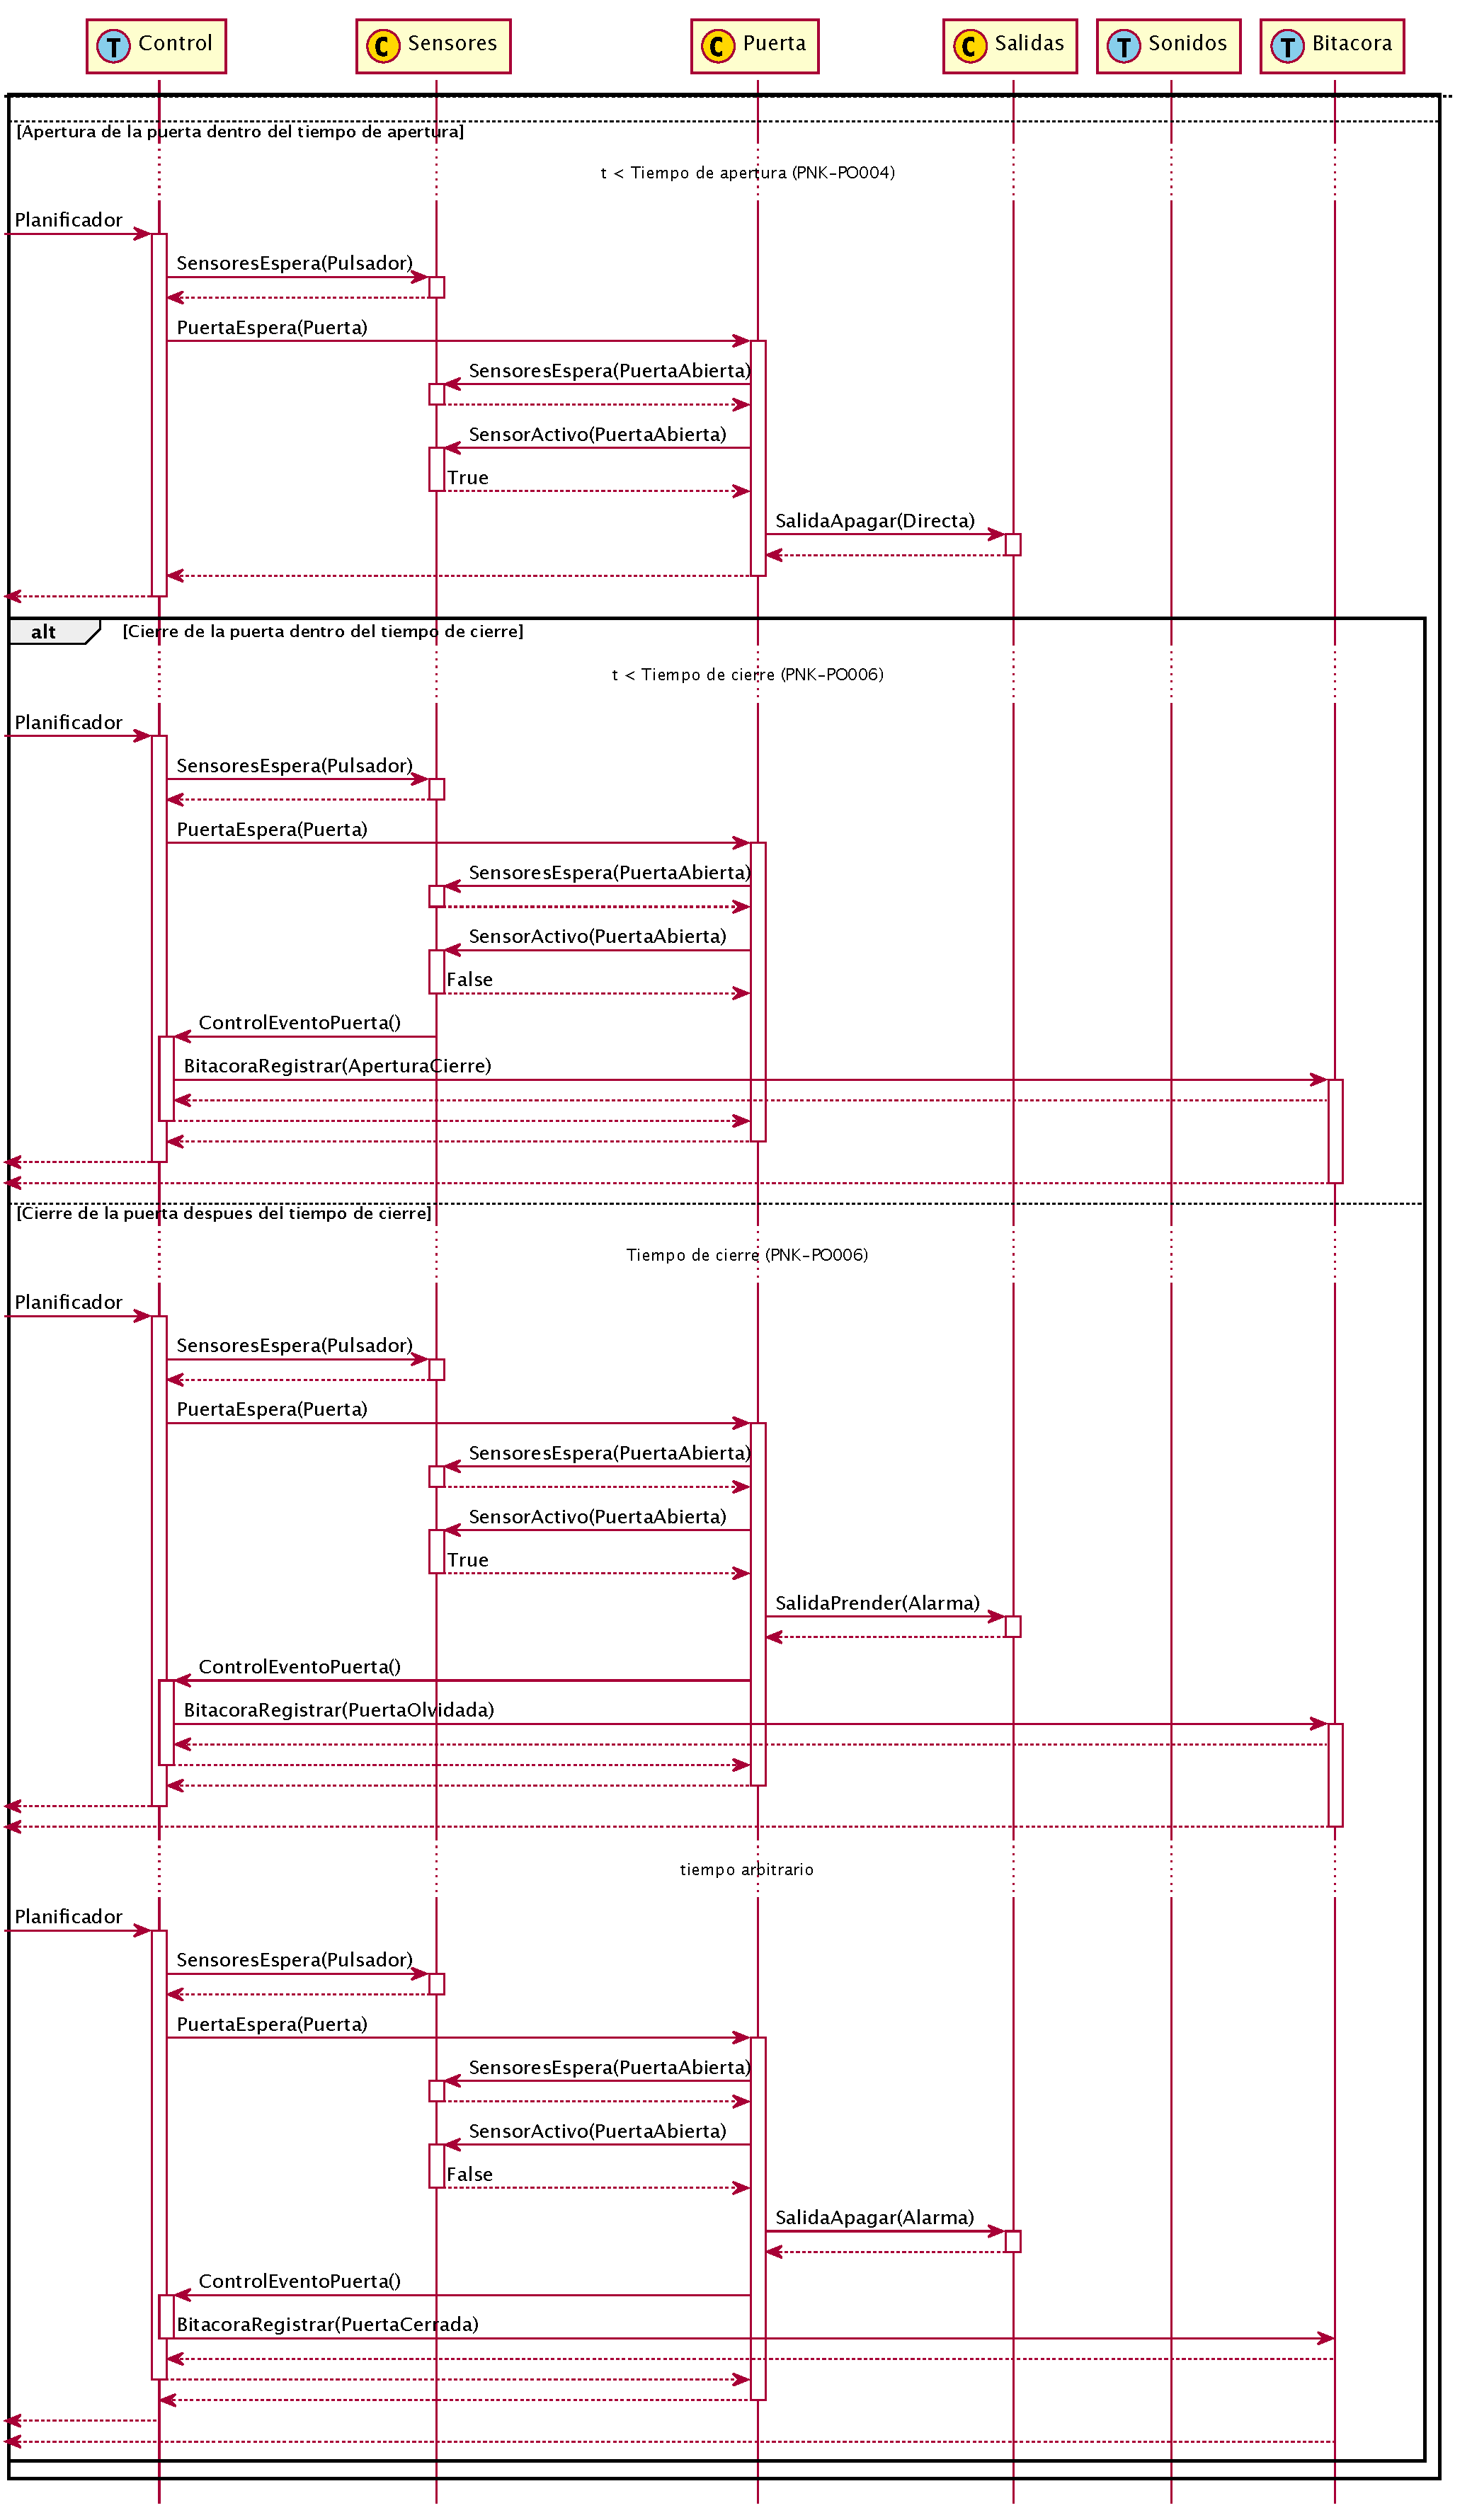
\includegraphics[width=\textwidth]{Figures/PNK-DS002-B.pdf}
	{\color{red} No es el diagrama correcto pero tiene la misma forma y extensión}
	\caption{Diagrama de secuencia para el cambio de configuración del equipo}
	\label{fig:SecuenciaConfiguracion}
\end{figure}

\FloatBarrier

\section{Desarrollo del firmware}
\label{sec:desarrollo}

\subsection{Entorno de desarrollo}

Se describen las herramientas utilizadas para el desarrollo del software

\begin{table}[ht]
	\centering
	\caption{Lista de las herramientas utilizadas para el desarrollo del firmware}
	\begin{tabular}{l c}    
		\toprule
		\textbf{Nombre} 	& \textbf{Característica}	\\
		\midrule
		Elemento 			& Valor	\\
		\bottomrule
		\hline
	\end{tabular}
	\label{tab:HerramientasDesarrollo}
\end{table}

\subsection{Uso del tipo de abstracto de datos}

Se presenta el patrón de programación denominado tipo abstracto de datos y se explica su uso en la implementación del firmware del equipo

\subsection{Pruebas de integración en las tareas del sistema}

Se presenta la problemática de implementar pruebas automatizadas en tareas del sistema operativo FreeRTOS y se explica la herramienta desarrollada para resolver este problema
